\subsection{Обзор существующих работ по анализу трафика}

3.2.1  Экспертные системы\par 

Как правило, экспертные системы создаются для решения практических задач в некоторых узкоспециализированных областях, где большую роль играют знания «бывалых» специалистов. Экспертные системы были первыми разработками, которые смогли привлечь большое внимание к результатам исследований в области искусственного интеллекта.\par 

Экспертные системы имеют одно большое отличие от других систем искусственного интеллекта: они не предназначены для решения каких-то универсальных задач, как например нейронные сети или генетические алгоритмы. Экспертные системы предназначены для качественного решения задач в определенной разработчиками области, в редких случаях – областях.\par 

Дороти Деннинг, при содействии Питера Неймана, опубликовали модель СОВ в 1986, сформировавшую основу для большинства современных систем. Её модель использовала статистические методы для обнаружения вторжений и называлась IDES (Intrusion detection expert system — экспертная система обнаружения вторжений). Система работала на рабочих станциях Sun и проверяла как сетевой трафик, так и данные пользовательских приложений. IDES использовала два подхода к обнаружению вторжений: в ней использовалась экспертная система для определения известных видов вторжений и компонент обнаружения, основанный на статистических методах и профилях пользователей и систем охраняемой сети.\par 

Самым крупным недостатком экспертной системы в качестве системы обнаружения вторжений является неспособность в принципе обнаруживать новые виды атак. Кроме того, известно множество технологий обхода систем обнаружения вторжений на основе экспертных систем, например, polymorphic shell code, insertion, exclusion и т.п.\par 

3.2.2  Искусственные нейронные сети\par 

Экспертные системы хорошо себя зарекомендовали, но только в узкоспециализированных областях. Для создания более универсальных интеллектуальных систем требовался другой подход. Наверное, это привело к тому, что исследователи искусственного интеллекта обратили внимание на биологические нейронные сети, которые лежат в основе человеческого мозга.\par 

Искусственная нейронная сеть – это математическая модель, а также её программная или аппаратная реализация, построенная по принципу организации и функционирования биологических нейронных сетей (сетей нервных клеток живого организма).\par 

Жигулин П.В. и Подворчан Д.Э. использовали для детектирования атак двухслойной персептрон с одним скрытым слоем по схеме 38 входных, 38 скрытых, 10 выходных нейронов . Точность определения типа атаки достигла 98\%. \par 

Исследователи Моради М. и Зелкернин М. из университета Queen использовали несколько схем реализации нейросети и получили следующие результаты:
\begin{itemize}
\item первая схема: 35 входных, 35 скрытых нейронов первого уровня, 35 скрытых нейронов второго уровня, 3 выходных нейрона показала 91\% верных решений на тестовых примерах;
\item вторая схема: 35 входных, 45 скрытых, 3 выходных нейронов показала 87\% верных решений на тестовых примерах;
\item третья схема: 41 входных, 40 скрытых нейронов первого уровня, 40 скрытых нейронов второго уровня, 1 выходной нейрон показала 99\% верных решений на тестовых примерах.
\end{itemize}

Третья схема с большой вероятностью определяет наличие атаки, но не ее тип.\par

Как видно из полученных результатов, увеличение числа скрытых слоев не приводит к значительному улучшению качества работы сети (всего 4\%) при экспоненциально возросшей сложности схемы и, как следствие, времени анализа.\par 

Исследователи Клионский Д.М., Большев А.К. и Геппенер В.В. разработали систему на основе HNIDS (Heuristic Network Intrusion Detection Systems), которая использует однослойный классификатор на базе искусственных нейронных сетей (ИНС).\par 

На рисунке \ref{img:2} представлена ИНС, реализующая работу однослойного классификатора. В качестве функции активации используется сигмоидальная функция активации где:
\begin{itemize}
\item h -- количество нейронов скрытого слоя;
\item n -- коэффициент скорости обучения;
\item m -- коэффициент инерционности.
\end{itemize}

\begin{figure}[h!]
    \centering
    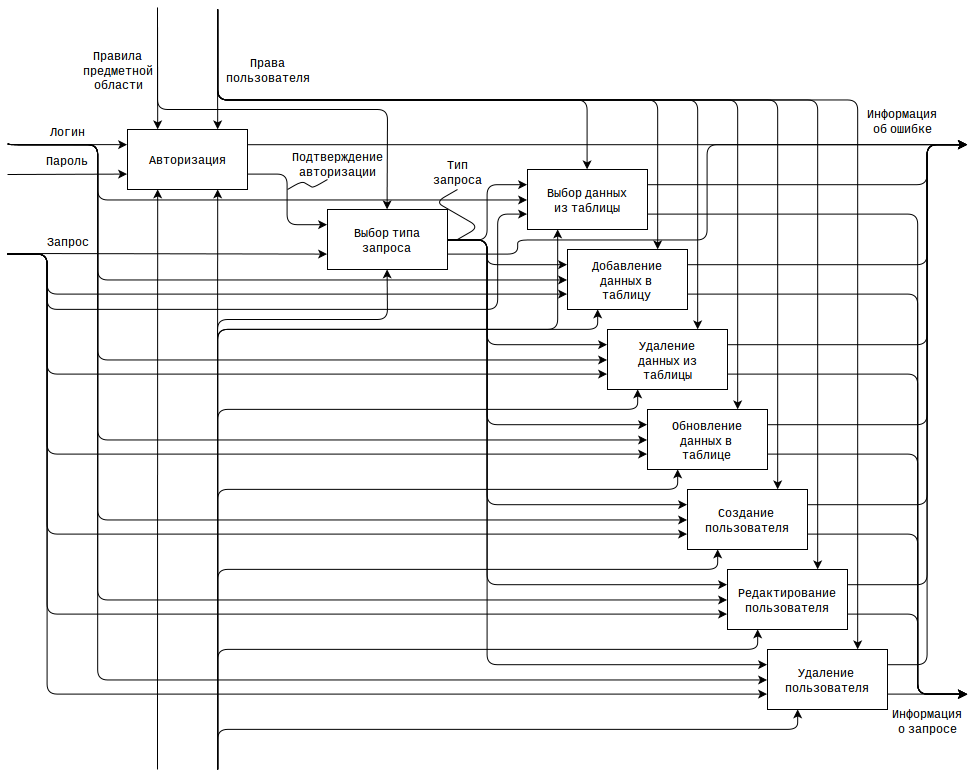
\includegraphics[width=0.55\textwidth]{2}
    \caption{Нейронная сеть, представляющая собой однослойный классификатор}
    \label{img:2}
\end{figure} 

Главным отличием такого типа систем от других является то, что система обучается на «нормальном» трафике целевой сети и в случае обнаружения отклонений сообщает об атаке или аномалии. Система работает на сетевом (транспортном) уровнях модели открытых систем и анализирует завершенные TCP-сессии между хостами.\par 

При тестировании прототипа исследователями в тестовой выборке использовали 17 вторжений сетевого уровня. С помощью варьирования параметров ИНС проводились минимизации по критериям ложной тревоги (FP) и пропуска сигналов (FN). При минимизации по критерию FP, прототип обнаружил 12 атак при 2 ложных срабатываниях.\par 

При минимизации по критерию FN, прототип обнаружил 16 атак при 1878 ложных срабатываниях.\par 

В своих исследованиях Жульков Е.В. предложил разбить трафик на векторы и при помощи системы обнаружения вторжений (СОВ), построенной по модульному принципу, анализировать трафик как векторы. \par 

Вероятность обнаружения известных атак составила 91\%, вероятность обнаружения неизвестных атак составила 86\%.\par 

Хафизов А.Ф. предложил использовать гибридную нейронную сеть для анализа пифограмм атак. На первом этапе работы гибридной искусственной нейросети, на множестве входных векторов обучается слой Кохонена. В результате нейроны этого слоя самоорганизуются таким образом, что векторы их весов наилучшим образом отображают распределение данных обучающих векторов. Далее веса фиксируются и на вход подается обучающая выборка, затем происходит финальная корректировка весов нейронов. На втором этапе обучается персептронная сеть. Обучение происходит с учителем. Для данной сети обучающие сигналы формируются из выходных сигналов слоя Кохонена и вектора ожидаемых значений.\par 

Результатом работы такой нейронной сети является отнесение входных данных к классу атак или к классу нормальных взаимодействий.\par 

3.2.3  Нечеткие системы\par 

Нечеткие системы также нашли свое применение в качестве компонента системы обнаружения вторжений, так как они оперируют <<нечеткими>> и <<размытыми>> данными, которыми и являются векторы атак на вычислительные сети. В качестве примера применения нечетких систем в IDS, рассмотрим несколько работ отечественных и иностранных ученых.
Исследователи из Индии Шанмагавадива Р. и Нагаражан Н. создали систему обнаружения вторжений на основе нечеткой логики. Схема работы сети представлена на рисунке \ref{img:3}.\par

\begin{figure}[h!]
    \centering
    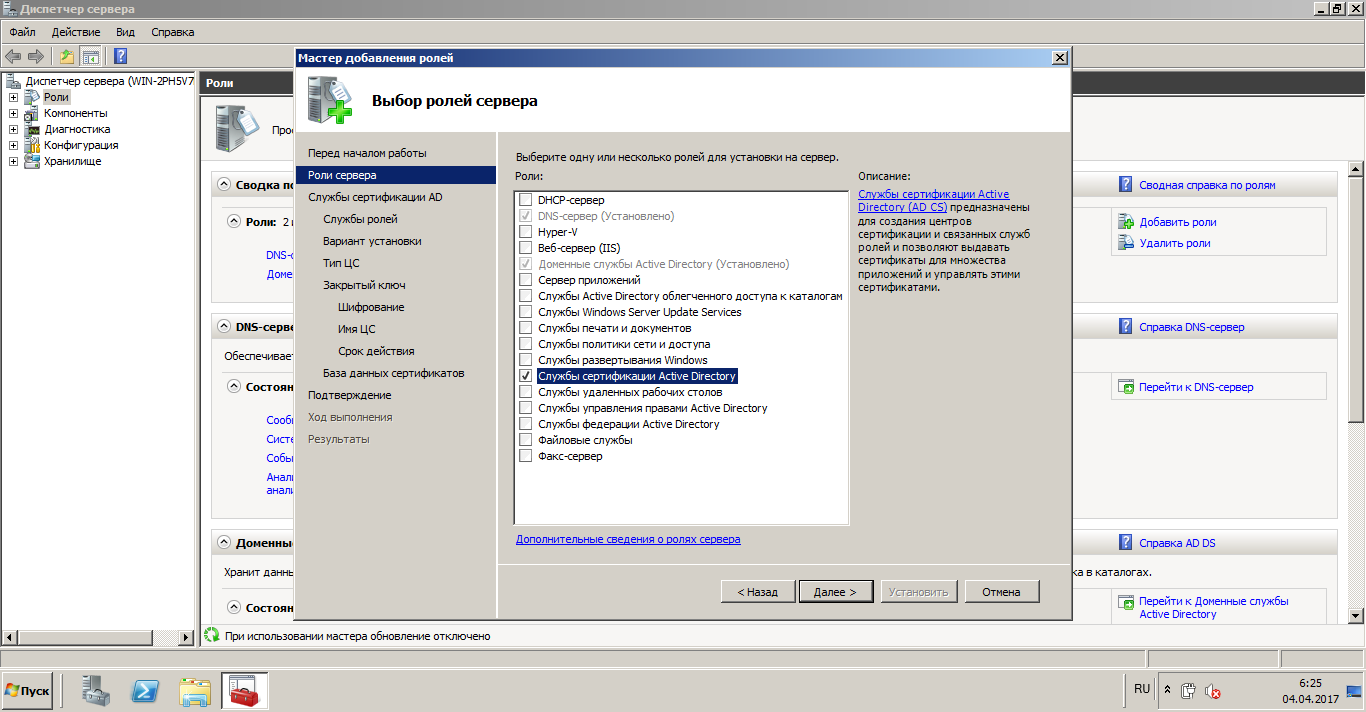
\includegraphics[width=0.65\textwidth]{3}
    \caption{Схема работы СОВ на основе нечеткой логики}
    \label{img:3}
\end{figure} 

Авторам удалось достичь более 90\% срабатываний, причем лишь 10\% набора использовалось для создания базы нечетких правил.\par 

Исследователи Слеповичев И.И.,  Ирматов П.В.,  Комарова М.С.  и Бежин А.А. разработали систему обнаружения SYN  Flood  атак на основе нечеткой нейронной сети.Метод обучения ИНС - метод обратного распространения ошибки.\par 

На основании разработанной модели исследователями была разработана программа, которая, используя математический аппарат нечеткой логики и нейронных сетей, определяет степень уверенности в наличии атаки.\par 

При синтезе алгоритмов активного аудита информационной системы Кашаевым Т.Р. была разработана система обнаружения вторжений на основе искусственных иммунных систем.\par 

Разработанная система использует нечеткие сети Петри. Система в общем случае работает следующим образом:
\begin{itemize}
\item определяются нормальные шаблоны активности системы (множество S) в виде строк равной длины l, составленных из букв конечного алфавита;
\item генерируется набор детекторов R, каждый из которых не совпадает ни с одной из строк из нормального шаблона активности. При этом кандидат в детекторы считается совпадающим с нормальным шаблоном в том и только в том случае, когда совпадают символы в r одинаковых позициях. Величина r подбирается в соответствии с решаемой задачей;
\item данные контролируются путем сопоставления детекторов с поведением системы. Любое совпадение на данном шаге означает изменение в работе системы (аномалию).
\end{itemize}

На основании разработанной модели был реализован прототип. Тестирование показало, что система обнаруживает до 85\% атак.\par 

3.2.4  Генетические алгоритмы\par 

Генетические алгоритмы предназначены для поиска оптимального решения на основе механизма естественного отбора в популяции. Популяция представляет собой множество хромосом, каждая из которых моделируется в виде битовой строки. Популяция развивается на основе трёх генетических операций – скрещивания, селекции и мутации. Развитие популяции продолжается до тех пор, пока не будет достигнут заданный критерий оптимальности, который определяется в виде специальной функции. В случае применения генетических алгоритмов для выявления атак в качестве элементов популяции выступают вектора определённой длины, каждый элемент которых соответствует определённой атаке. В результаты развития такой популяции можно получить оптимальный вектор, который будет указывать на то, какие атаки происходят в системе в текущий момент времени.\par 

Ученые Ануп Гоял и Четан Камар создали систему обнаружения вторжений GA-NIDS, основанную на генетическом алгоритме. Схема работы системы представлена на рисунке \ref{img:4}.

\clearpage

\begin{figure}[h!]
    \centering
    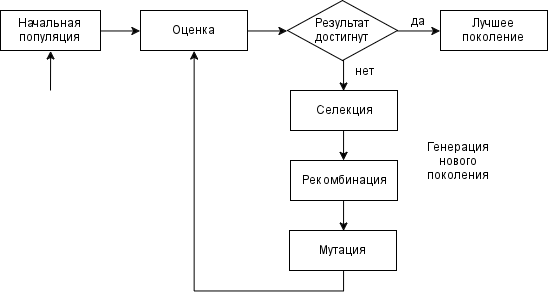
\includegraphics[width=0.8\textwidth]{4}
    \caption{Схема работы GA-NIDS}
    \label{img:4}
\end{figure} 

Для генерации правил использовалось 10\% набора KDD CUP 99. Сгенерированные правила показали более 95\% правильных решений на тестовых примерах.\par

3.2.5  Результат исследования\par 

В результате проведенного исследования было решено использовать искуственные нейронный сети для системы обнаружения вторжений. \par 

Первое преимущество в использовании нейронной сети в выявлении вторжений --- это гибкость, которую предоставляет эта сеть. Нейронная сеть способна анализировать данные из сети, даже если данные неполные или искажены. Кроме того, сеть будет обладать способностью проводить анализ с данными в нелинейной форме. Обе эти характеристики имеют важное значение в сетевой среде, где полученная информация подвержена случайным ошибкам системы. Кроме того, поскольку некоторые атаки на сеть могут быть проведены скоординированным вторжением нескольких злоумышленников, способность обрабатывать данные из нескольких источников в нелинейной форме особенно важна.\par 

Скорость, свойственная нейронным сетям, является еще одним преимуществом этого подхода. Поскольку защита вычислительных ресурсов требует своевременного выявления атак, скорость обработки нейронной сети может обеспечить реагирование на вторжение до того, как будет нанесен непоправимый ущерб системе.\par 

Поскольку результат работы нейронной сети выражается в виде вероятности, нейронная сеть обеспечивает возможность прогнозирования для обнаружения случаев вторжения. Система обнаружения вторжений на основе нейронных сетей определит вероятность того, что конкретное событие или ряд событий, свидетельствуют о нападении на систему. По мере получения опыта, нейронная сеть улучшает способность определять, какие события и где могут произойти в процессе атаки. Эта информация затем может быть использована, чтобы сгенерировать последовательность событий, которые должны произойти, если имеет место быть попытка вторжения. Отслеживая последующие возникновения этих событий, система будет способна улучшить анализ событий и, возможно, провести защитные меры, прежде чем атака будет удачно выполнена.\par 

Тем не менее, наиболее важным преимуществом нейронных сетей в выявлении вторжений является  способность нейронной сети <<обучаться>> признакам атак и определять случаи, которые нехарактерны для тех, что наблюдались ранее. Нейронная сеть может быть обучена распознавать известные подозрительные события с высокой степенью точности. Это очень ценное умение (злоумышленники часто повторяют <<успехи>> других) так же позволит получить возможность применять эти знания для выявления фактов о нападении, которые не соответствуют точным характеристикам предыдущих вторжений. Вероятность вторжения в систему может быть предполагаемая и помечена как потенциальная угроза, когда вероятность превышает определенный порог.\par 
